%=======================================================================
%  VRPSPDTW-E (EVRP-TW-SPD) — Paper breve IEEE
%  Trabajo Final — Optimizacion CINF105 — Universidad Andres Bello — 2026-1
%  Compilar en Overleaf:  pdfLaTeX  ->  BibTeX  ->  pdfLaTeX x2
%=======================================================================
\documentclass[conference]{IEEEtran}
\IEEEoverridecommandlockouts

\usepackage[T1]{fontenc}
\usepackage[utf8]{inputenc}
% --- Localizacion al espanol SIN babel (maxima portabilidad de compilacion).
%     Si tu Overleaf/distribucion soporta babel-spanish, puedes reemplazar
%     este bloque por:  \usepackage[spanish]{babel}
\renewcommand{\abstractname}{Resumen}
\renewcommand{\IEEEkeywordsname}{Palabras clave}
\renewcommand{\figurename}{Fig.}
\renewcommand{\tablename}{Tabla}
\renewcommand{\refname}{Referencias}
\usepackage{amsmath,amssymb,amsfonts}
\usepackage{graphicx}
\usepackage{booktabs}
\usepackage{array}
\usepackage{caption}
\usepackage{cite}
\usepackage{url}
\usepackage{tikz}
\usetikzlibrary{positioning,arrows.meta,calc,shapes.geometric,fit,backgrounds}

\begin{document}

\title{VRPSPDTW-E: Ruteo de Veh\'iculos El\'ectricos con Recogida y Entrega
Simult\'aneas y Ventanas de Tiempo --- Revisi\'on del Estado del Arte y el Rol de LKH-3}

\author{
\IEEEauthorblockN{Javier Far\'ias \quad Uriel Navarrete \quad Vicente Abarca}
\IEEEauthorblockA{\textit{Facultad de Ingenier\'ia, Universidad Andr\'es Bello}, Santiago, Chile \\
CINF105 --- Optimizaci\'on, Per\'iodo 2026-1 \\
j.farascrcamo@uandresbello.edu \quad u.navarretecadima@uandresbello.edu \\
v.abarcapalacios@uandresbello.edu}
}

\maketitle

%-----------------------------------------------------------------------
\begin{abstract}
El \emph{Vehicle Routing Problem with Simultaneous Pickup-Delivery and Time
Windows} (VRPSPDTW) es una variante de ruteo soportada por el solver LKH-3 de
Helsgaun. Este trabajo aborda su extensi\'on a \emph{veh\'iculos el\'ectricos}
(VRPSPDTW-E, conocida como EVRP-TW-SPD), donde la autonom\'ia limitada obliga a
recargar en estaciones durante la ruta. Presentamos la definici\'on formal y una
formulaci\'on MILP con objetivo multi-criterio (veh\'iculos, distancia, energ\'ia
y tiempo) y consumo \emph{dependiente de la carga}; analizamos su complejidad
(NP-hard) y tres aplicaciones reales (e-commerce con log\'istica inversa,
distribuci\'on urbana verde y reciclaje). Revisamos cr\'iticamente el estado del
arte ---exactos, heur\'isticos, metaheur\'isticos (memet\'icos, CMSA, ALNS) y de
aprendizaje--- y posicionamos a LKH-3: resuelve nativamente el n\'ucleo VRPSPDTW
con alta calidad, pero \emph{no} modela la capa el\'ectrica y escala mal en
tiempo. Proponemos usarlo como motor base envuelto en una capa de inserci\'on de
estaciones y recarga parcial, y cerramos con brechas abiertas y tendencias
recientes.
\end{abstract}

\begin{IEEEkeywords}
ruteo de veh\'iculos, veh\'iculos el\'ectricos, recogida y entrega
simult\'aneas, ventanas de tiempo, LKH-3, optimizaci\'on combinatorial.
\end{IEEEkeywords}

%=======================================================================
\section{Introducci\'on y motivaci\'on}
%=======================================================================
La \'ultima milla concentra una fracci\'on creciente del costo log\'istico y de
las emisiones urbanas. Tres tendencias la transforman simult\'aneamente: la
\emph{electrificaci\'on} de flotas (impulsada por zonas de bajas emisiones), la
\emph{log\'istica inversa} (devoluciones, envases y reciclaje que viajan del
cliente al dep\'osito) y la exigencia de \emph{ventanas de tiempo} pactadas con
el cliente \cite{koc2020review,kucukoglu2021review}. Su confluencia da lugar al
\emph{Vehicle Routing Problem with Simultaneous Pickup-Delivery and Time Windows}
con veh\'iculos el\'ectricos, que abreviamos \textbf{VRPSPDTW-E} (equivalente al
EVRP-TW-SPD de la literatura reciente \cite{akbay2022cmsa,zheng2025hma}).
Operadores como JD Logistics y CAINIAO operan exactamente bajo este esquema, con
instancias de cientos a miles de clientes \cite{zheng2025hma,liu2021mate}.

El problema base, VRPSPDTW, figura entre las variantes que resuelve el solver
LKH-3 (Lin--Kernighan--Helsgaun, versi\'on 3) \cite{helsgaun2017lkh3}, uno de los
mejores resolvedores heur\'isticos para la familia TSP/VRP. Sin embargo, la
componente el\'ectrica ---autonom\'ia, estaciones de carga y recarga parcial---
queda \emph{fuera} del alcance nativo de LKH-3. Esta brecha estructura nuestro
an\'alisis cr\'itico. Las contribuciones de este trabajo de revisi\'on son:
(i)~una definici\'on formal y una MILP unificada del VRPSPDTW-E
(Secci\'on~\ref{sec:form}); (ii)~su an\'alisis de complejidad y aplicaciones
(Secci\'on~\ref{sec:comp}); (iii)~una revisi\'on cr\'itica del estado del arte
que posiciona a LKH-3 (Secciones~\ref{sec:sota} y \ref{sec:lkh}); y
(iv)~la identificaci\'on de brechas abiertas (Secci\'on~\ref{sec:gaps}).

%=======================================================================
\section{Definici\'on formal y formulaci\'on}\label{sec:form}
%=======================================================================
\subsection{Del problema base a la variante el\'ectrica}
En el VRPSPDTW, una flota de veh\'iculos id\'enticos parte de un dep\'osito y
atiende a cada cliente \emph{en una sola visita}, \emph{entregando} mercanc\'ia
tra\'ida del dep\'osito y \emph{recogiendo} simult\'aneamente mercanc\'ia que
debe retornar a \'el, dentro de una ventana de tiempo \cite{min1989,dethloff2001}.
El rasgo cr\'itico del \emph{simultaneous pickup-delivery} (SPD) es que la carga
a bordo var\'ia de forma \emph{no mon\'otona}: el veh\'iculo sale cargado con
todas las entregas y regresa cargado con todas las recogidas, de modo que la
capacidad debe respetarse en \emph{todo} punto de la ruta.

La variante el\'ectrica a\~nade tres elementos
(Fig.~\ref{fig:esquema}, Tabla~\ref{tab:diff}): un conjunto de
\emph{estaciones de carga} (visitables varias veces), una variable de estado
adicional ---el \emph{estado de carga} (SoC) de la bater\'ia, que debe
mantenerse no negativo--- y una decisi\'on continua de \emph{cu\'anto recargar}
(recarga parcial), que consume tiempo e interact\'ua con las ventanas
\cite{schneider2014evrptw,keskin2016partial}.

\begin{center}
\captionof{table}{Qu\'e a\~nade la ``E'' al problema soportado por LKH-3.}
\label{tab:diff}
\renewcommand{\arraystretch}{1.15}
\begin{tabular}{@{}lcc@{}}
  \toprule
  Caracter\'istica & VRPSPDTW & VRPSPDTW-E \\
  \midrule
  Carga no mon\'otona (SPD) & s\'i & s\'i \\
  Ventanas de tiempo & s\'i & s\'i \\
  Capacidad de carga & s\'i & s\'i \\
  Autonom\'ia / bater\'ia (SoC) & \textbf{no} & \textbf{s\'i} \\
  Estaciones de carga & \textbf{no} & \textbf{s\'i} \\
  Recarga parcial & \textbf{no} & \textbf{s\'i} \\
  \midrule
  Soportado por LKH-3 & \textbf{s\'i} & \textbf{no} \\
  \bottomrule
\end{tabular}
\end{center}

\begin{figure}[t]
  \centering
  \resizebox{\columnwidth}{!}{% fig1_esquema.tex  — Figura 1: esquema del problema VRPSPDTW-E
% Requiere en el preámbulo del documento que la incluye:
%   \usetikzlibrary{positioning,arrows.meta,calc,shapes.geometric}
% Se incluye con:  % fig1_esquema.tex  — Figura 1: esquema del problema VRPSPDTW-E
% Requiere en el preámbulo del documento que la incluye:
%   \usetikzlibrary{positioning,arrows.meta,calc,shapes.geometric}
% Se incluye con:  % fig1_esquema.tex  — Figura 1: esquema del problema VRPSPDTW-E
% Requiere en el preámbulo del documento que la incluye:
%   \usetikzlibrary{positioning,arrows.meta,calc,shapes.geometric}
% Se incluye con:  \input{fig1_esquema}
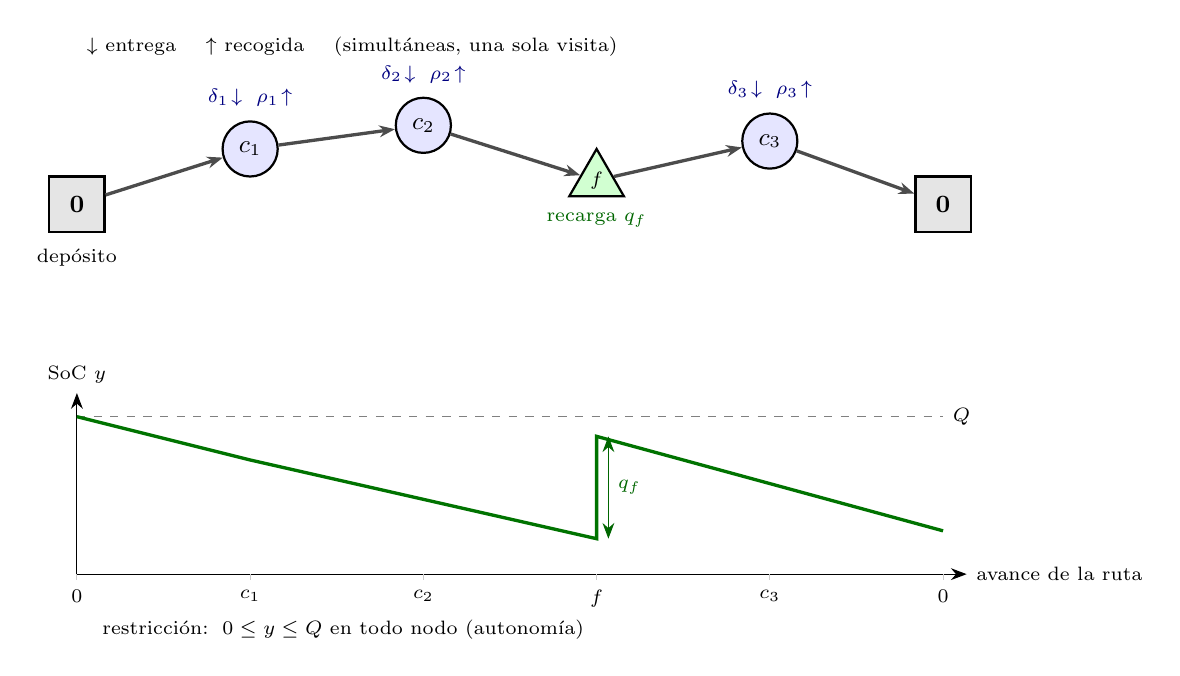
\begin{tikzpicture}[
  >={Stealth[length=2mm]},
  depot/.style={rectangle,draw,thick,fill=gray!20,minimum size=7mm,font=\small\bfseries},
  cust/.style={circle,draw,thick,fill=blue!10,minimum size=7mm,font=\small},
  stat/.style={regular polygon,regular polygon sides=3,draw,thick,fill=green!18,
               minimum size=8mm,inner sep=0pt,font=\scriptsize},
  arc/.style={->,very thick,gray!60!black}
]
  % ---------- Ruta (parte superior) ----------
  \node[depot] (d0) at (0,0)   {0};
  \node[cust]  (c1) at (2.2,0.7) {$c_1$};
  \node[cust]  (c2) at (4.4,1.0) {$c_2$};
  \node[stat]  (f)  at (6.6,0.3) {$f$};
  \node[cust]  (c3) at (8.8,0.8) {$c_3$};
  \node[depot] (d1) at (11,0)  {0};

  \draw[arc] (d0) -- (c1);
  \draw[arc] (c1) -- (c2);
  \draw[arc] (c2) -- (f);
  \draw[arc] (f)  -- (c3);
  \draw[arc] (c3) -- (d1);

  % etiquetas entrega (delivery) y recogida (pickup) simultaneas
  \node[font=\scriptsize,blue!50!black,above=0.5mm of c1] {$\delta_1\!\downarrow\ \rho_1\!\uparrow$};
  \node[font=\scriptsize,blue!50!black,above=0.5mm of c2] {$\delta_2\!\downarrow\ \rho_2\!\uparrow$};
  \node[font=\scriptsize,blue!50!black,above=0.5mm of c3] {$\delta_3\!\downarrow\ \rho_3\!\uparrow$};
  \node[font=\scriptsize,green!40!black,below=0.8mm of f] {recarga $q_f$};
  \node[font=\scriptsize,below=0.8mm of d0] {dep\'osito};

  % leyenda compacta
  \node[font=\scriptsize,anchor=west] at (0,2.0)
    {$\downarrow$ entrega \quad $\uparrow$ recogida \quad (simult\'aneas, una sola visita)};

  % ---------- Curva de estado de carga SoC (parte inferior) ----------
  \begin{scope}[yshift=-4.7cm]
    \draw[->] (0,0) -- (11.3,0) node[right,font=\scriptsize] {avance de la ruta};
    \draw[->] (0,0) -- (0,2.3) node[above,font=\scriptsize] {SoC $y$};
    \draw[dashed,gray] (0,2.0) -- (11,2.0) node[right,font=\scriptsize,black] {$Q$};

    % SoC: parte llena en 0, baja con la distancia, salta en la estacion f, vuelve a bajar
    \draw[very thick,green!45!black]
      (0,2.0) -- (2.2,1.45) -- (4.4,0.95) -- (6.6,0.45) % consumo hasta la estacion
      -- (6.6,1.75)                                      % salto por recarga parcial q_f
      -- (8.8,1.15) -- (11,0.55);                        % consumo hasta el deposito

    % marcas verticales de los nodos
    \foreach \x/\lab in {0/0,2.2/c_1,4.4/c_2,6.6/f,8.8/c_3,11/0}
      \draw[gray!40] (\x,0) -- (\x,-0.08) node[below,font=\scriptsize,black] {$\lab$};

    \draw[<->,green!40!black] (6.75,0.45) -- (6.75,1.75)
      node[midway,right,font=\scriptsize] {$q_f$};
    \node[font=\scriptsize,anchor=west] at (0.2,-0.7)
      {restricci\'on: $\,0 \le y \le Q$ en todo nodo (autonom\'ia)};
  \end{scope}
\end{tikzpicture}

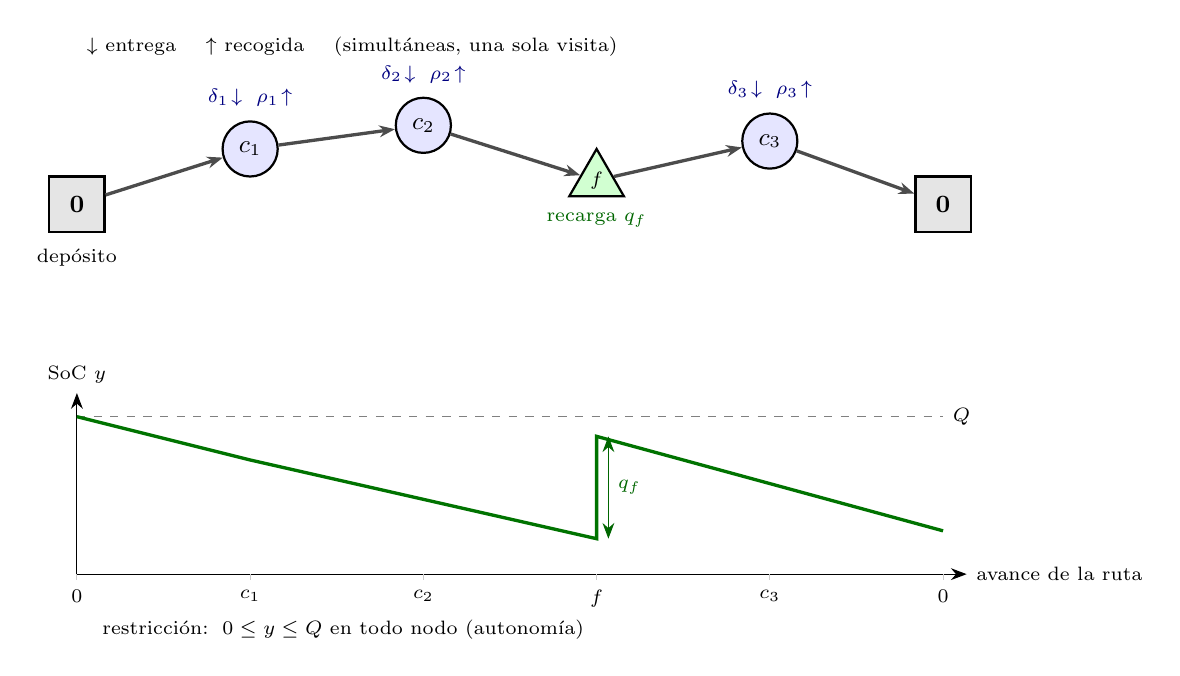
\begin{tikzpicture}[
  >={Stealth[length=2mm]},
  depot/.style={rectangle,draw,thick,fill=gray!20,minimum size=7mm,font=\small\bfseries},
  cust/.style={circle,draw,thick,fill=blue!10,minimum size=7mm,font=\small},
  stat/.style={regular polygon,regular polygon sides=3,draw,thick,fill=green!18,
               minimum size=8mm,inner sep=0pt,font=\scriptsize},
  arc/.style={->,very thick,gray!60!black}
]
  % ---------- Ruta (parte superior) ----------
  \node[depot] (d0) at (0,0)   {0};
  \node[cust]  (c1) at (2.2,0.7) {$c_1$};
  \node[cust]  (c2) at (4.4,1.0) {$c_2$};
  \node[stat]  (f)  at (6.6,0.3) {$f$};
  \node[cust]  (c3) at (8.8,0.8) {$c_3$};
  \node[depot] (d1) at (11,0)  {0};

  \draw[arc] (d0) -- (c1);
  \draw[arc] (c1) -- (c2);
  \draw[arc] (c2) -- (f);
  \draw[arc] (f)  -- (c3);
  \draw[arc] (c3) -- (d1);

  % etiquetas entrega (delivery) y recogida (pickup) simultaneas
  \node[font=\scriptsize,blue!50!black,above=0.5mm of c1] {$\delta_1\!\downarrow\ \rho_1\!\uparrow$};
  \node[font=\scriptsize,blue!50!black,above=0.5mm of c2] {$\delta_2\!\downarrow\ \rho_2\!\uparrow$};
  \node[font=\scriptsize,blue!50!black,above=0.5mm of c3] {$\delta_3\!\downarrow\ \rho_3\!\uparrow$};
  \node[font=\scriptsize,green!40!black,below=0.8mm of f] {recarga $q_f$};
  \node[font=\scriptsize,below=0.8mm of d0] {dep\'osito};

  % leyenda compacta
  \node[font=\scriptsize,anchor=west] at (0,2.0)
    {$\downarrow$ entrega \quad $\uparrow$ recogida \quad (simult\'aneas, una sola visita)};

  % ---------- Curva de estado de carga SoC (parte inferior) ----------
  \begin{scope}[yshift=-4.7cm]
    \draw[->] (0,0) -- (11.3,0) node[right,font=\scriptsize] {avance de la ruta};
    \draw[->] (0,0) -- (0,2.3) node[above,font=\scriptsize] {SoC $y$};
    \draw[dashed,gray] (0,2.0) -- (11,2.0) node[right,font=\scriptsize,black] {$Q$};

    % SoC: parte llena en 0, baja con la distancia, salta en la estacion f, vuelve a bajar
    \draw[very thick,green!45!black]
      (0,2.0) -- (2.2,1.45) -- (4.4,0.95) -- (6.6,0.45) % consumo hasta la estacion
      -- (6.6,1.75)                                      % salto por recarga parcial q_f
      -- (8.8,1.15) -- (11,0.55);                        % consumo hasta el deposito

    % marcas verticales de los nodos
    \foreach \x/\lab in {0/0,2.2/c_1,4.4/c_2,6.6/f,8.8/c_3,11/0}
      \draw[gray!40] (\x,0) -- (\x,-0.08) node[below,font=\scriptsize,black] {$\lab$};

    \draw[<->,green!40!black] (6.75,0.45) -- (6.75,1.75)
      node[midway,right,font=\scriptsize] {$q_f$};
    \node[font=\scriptsize,anchor=west] at (0.2,-0.7)
      {restricci\'on: $\,0 \le y \le Q$ en todo nodo (autonom\'ia)};
  \end{scope}
\end{tikzpicture}

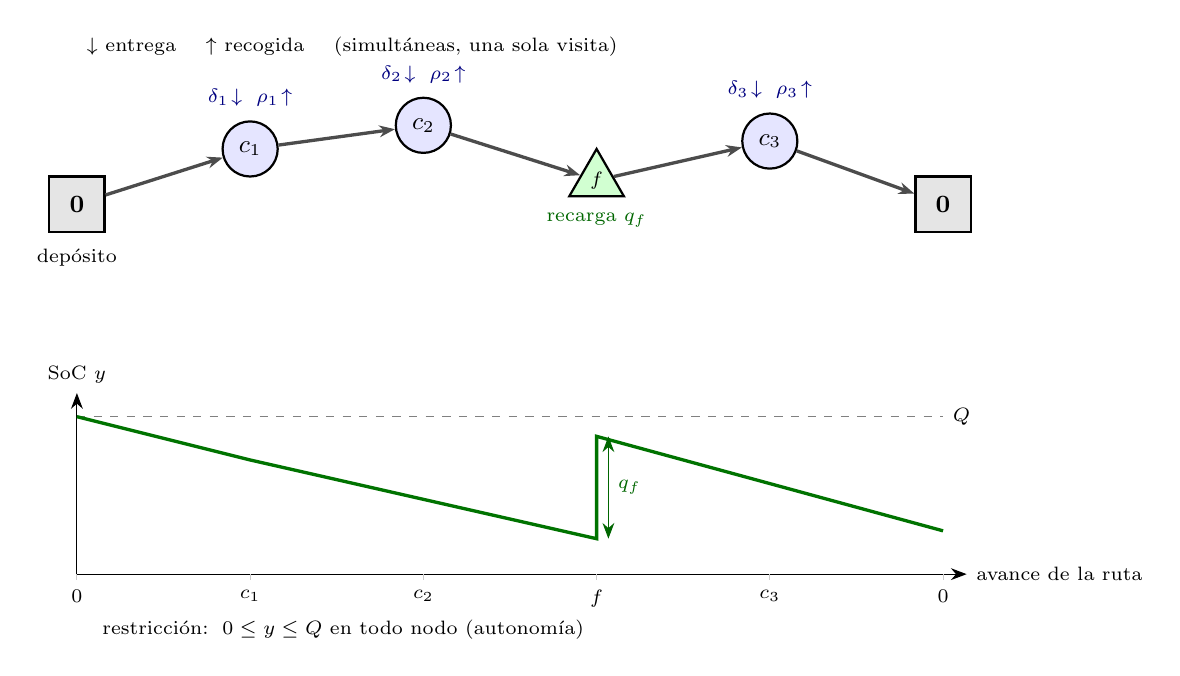
\begin{tikzpicture}[
  >={Stealth[length=2mm]},
  depot/.style={rectangle,draw,thick,fill=gray!20,minimum size=7mm,font=\small\bfseries},
  cust/.style={circle,draw,thick,fill=blue!10,minimum size=7mm,font=\small},
  stat/.style={regular polygon,regular polygon sides=3,draw,thick,fill=green!18,
               minimum size=8mm,inner sep=0pt,font=\scriptsize},
  arc/.style={->,very thick,gray!60!black}
]
  % ---------- Ruta (parte superior) ----------
  \node[depot] (d0) at (0,0)   {0};
  \node[cust]  (c1) at (2.2,0.7) {$c_1$};
  \node[cust]  (c2) at (4.4,1.0) {$c_2$};
  \node[stat]  (f)  at (6.6,0.3) {$f$};
  \node[cust]  (c3) at (8.8,0.8) {$c_3$};
  \node[depot] (d1) at (11,0)  {0};

  \draw[arc] (d0) -- (c1);
  \draw[arc] (c1) -- (c2);
  \draw[arc] (c2) -- (f);
  \draw[arc] (f)  -- (c3);
  \draw[arc] (c3) -- (d1);

  % etiquetas entrega (delivery) y recogida (pickup) simultaneas
  \node[font=\scriptsize,blue!50!black,above=0.5mm of c1] {$\delta_1\!\downarrow\ \rho_1\!\uparrow$};
  \node[font=\scriptsize,blue!50!black,above=0.5mm of c2] {$\delta_2\!\downarrow\ \rho_2\!\uparrow$};
  \node[font=\scriptsize,blue!50!black,above=0.5mm of c3] {$\delta_3\!\downarrow\ \rho_3\!\uparrow$};
  \node[font=\scriptsize,green!40!black,below=0.8mm of f] {recarga $q_f$};
  \node[font=\scriptsize,below=0.8mm of d0] {dep\'osito};

  % leyenda compacta
  \node[font=\scriptsize,anchor=west] at (0,2.0)
    {$\downarrow$ entrega \quad $\uparrow$ recogida \quad (simult\'aneas, una sola visita)};

  % ---------- Curva de estado de carga SoC (parte inferior) ----------
  \begin{scope}[yshift=-4.7cm]
    \draw[->] (0,0) -- (11.3,0) node[right,font=\scriptsize] {avance de la ruta};
    \draw[->] (0,0) -- (0,2.3) node[above,font=\scriptsize] {SoC $y$};
    \draw[dashed,gray] (0,2.0) -- (11,2.0) node[right,font=\scriptsize,black] {$Q$};

    % SoC: parte llena en 0, baja con la distancia, salta en la estacion f, vuelve a bajar
    \draw[very thick,green!45!black]
      (0,2.0) -- (2.2,1.45) -- (4.4,0.95) -- (6.6,0.45) % consumo hasta la estacion
      -- (6.6,1.75)                                      % salto por recarga parcial q_f
      -- (8.8,1.15) -- (11,0.55);                        % consumo hasta el deposito

    % marcas verticales de los nodos
    \foreach \x/\lab in {0/0,2.2/c_1,4.4/c_2,6.6/f,8.8/c_3,11/0}
      \draw[gray!40] (\x,0) -- (\x,-0.08) node[below,font=\scriptsize,black] {$\lab$};

    \draw[<->,green!40!black] (6.75,0.45) -- (6.75,1.75)
      node[midway,right,font=\scriptsize] {$q_f$};
    \node[font=\scriptsize,anchor=west] at (0.2,-0.7)
      {restricci\'on: $\,0 \le y \le Q$ en todo nodo (autonom\'ia)};
  \end{scope}
\end{tikzpicture}
}
  \caption{Esquema del VRPSPDTW-E. Arriba: una ruta entrega ($\downarrow$) y
  recoge ($\uparrow$) en cada cliente y se desv\'ia a una estaci\'on $f$ para
  recargar $q_f$. Abajo: el estado de carga (SoC) decae con la distancia y se
  repone parcialmente en $f$, sujeto a $0\le y\le Q$.}
  \label{fig:esquema}
\end{figure}

\subsection{Notaci\'on}
Sea un grafo dirigido sobre los nodos $\mathcal{N}=\{0\}\cup\mathcal{V}\cup
\mathcal{F}'$, donde $0$ es el dep\'osito, $\mathcal{V}$ el conjunto de clientes
y $\mathcal{F}'$ un conjunto de \emph{copias} de las estaciones de carga (cada
estaci\'on se replica para admitir visitas m\'ultiples; cada copia se visita a lo
sumo una vez). Cada arco $(i,j)$ tiene distancia $d_{ij}$ y tiempo de viaje
$t_{ij}$. Cada cliente $i$ tiene demanda de entrega $\delta_i$, demanda de
recogida $\rho_i$, ventana $[e_i,l_i]$ y tiempo de servicio $s_i$; en el
dep\'osito y las estaciones $\delta_i=\rho_i=s_i=0$. La flota es homog\'enea con
capacidad de carga $C$ y de bater\'ia $Q$. El consumo de energ\'ia por unidad de
distancia tiene una parte fija $h_0$ y una parte $h_1$ \emph{proporcional a la
carga transportada} (un veh\'iculo el\'ectrico gasta m\'as cuanto m\'as pesa);
$g$ es el tiempo de recarga por unidad de energ\'ia. Los coeficientes
$\mu_1,\dots,\mu_4\ge0$ ponderan los cuatro criterios del costo ---veh\'iculos,
distancia, energ\'ia y tiempo--- en una unidad com\'un.

\emph{Variables de decisi\'on:} $x_{ij}\in\{0,1\}$ indica si se recorre el arco
$(i,j)$; $\tau_i\ge0$ es el instante de inicio de servicio en $i$; $y_i\ge0$ es
el SoC al llegar a $i$; $D_{ij}\ge0$ y $P_{ij}\ge0$ son, respectivamente, la
carga de entregas a\'un a bordo y de recogidas ya acumuladas al recorrer
$(i,j)$; y $q_i\ge0$ es la energ\'ia recargada en la estaci\'on $i\in\mathcal{F}'$.

\subsection{Formulaci\'on MILP}
La siguiente formulaci\'on integra la estructura de flujo del VRPSPD
\cite{dethloff2001} con el seguimiento de bater\'ia y tiempo del EVRPTW
\cite{schneider2014evrptw}:
\begin{align}
\min\;\; & \mu_1\!\!\sum_{j\in\mathcal{V}\cup\mathcal{F}'}\!\! x_{0j}
         + \mu_2\!\!\sum_{(i,j)}\! d_{ij} x_{ij}
         + \mu_3 E + \mu_4 T \label{eq:obj}\\
\text{s.a.}\;\;
& \textstyle\sum_{j} x_{ij}=1, && \forall i\in\mathcal{V} \label{eq:deg1}\\
& \textstyle\sum_{j} x_{ij}\le1, && \forall i\in\mathcal{F}' \label{eq:deg2}\\
& \textstyle\sum_{i} x_{ij}-\sum_{k} x_{jk}=0, && \forall j\in\mathcal{N} \label{eq:cons}\\
& D_{ij}+P_{ij}\le C\,x_{ij}, && \forall (i,j) \label{eq:cap}\\
& \textstyle\sum_{i} D_{ij}-\sum_{k} D_{jk}=\delta_j, && \forall j\in\mathcal{V} \label{eq:fd}\\
& \textstyle\sum_{k} P_{jk}-\sum_{i} P_{ij}=\rho_j, && \forall j\in\mathcal{V} \label{eq:fp}\\
& \tau_i+\sigma_i+t_{ij}-\tau_j\le M(1-x_{ij}), && \forall (i,j) \label{eq:time}\\
& e_i\le\tau_i\le l_i, && \forall i\in\mathcal{N} \label{eq:tw}\\
& y_j\le y_i+\gamma_i-\varepsilon_{ij}+Q(1-x_{ij}), && \forall (i,j) \label{eq:soc}\\
& 0\le y_i\le Q,\quad y_i+q_i\le Q, && \forall i \label{eq:socb}\\
& x_{ij}\in\{0,1\};\; \tau_i,y_i,q_i,D_{ij},P_{ij}\ge0. && \label{eq:dom}
\end{align}
donde $\varepsilon_{ij}=(h_0 x_{ij}+h_1(D_{ij}+P_{ij}))\,d_{ij}$ es la energ\'ia consumida
en el arco $(i,j)$ ---una parte fija m\'as una parte que crece con la carga a
bordo, que en SPD var\'ia a lo largo de la ruta---; $E=\sum_{(i,j)}\varepsilon_{ij}$ es la
energ\'ia total y $T=\sum_{(i,j)}t_{ij}x_{ij}+g\sum_{i\in\mathcal{F}'}q_i$ el
tiempo total de viaje m\'as recarga. Por compacidad, $\sigma_i=s_i$ y
$\gamma_i=0$ si $i\in\mathcal{V}$, mientras que $\sigma_i=g\,q_i$ y
$\gamma_i=q_i$ si $i\in\mathcal{F}'$ (en una estaci\'on el ``servicio'' es el
tiempo de recarga $g\,q_i$ y el SoC aumenta en $q_i$); en el dep\'osito
$y_0=Q$. $M$ es una constante suficientemente grande.

\emph{Interpretaci\'on.} La funci\'on objetivo \eqref{eq:obj} minimiza un costo
operativo que pondera cuatro criterios: n\'umero de veh\'iculos (costo fijo de
despacho), distancia recorrida, energ\'ia el\'ectrica consumida ($E$) y tiempo
total de viaje y recarga ($T$). \eqref{eq:deg1}--\eqref{eq:deg2} obligan a
visitar cada cliente una vez y
cada copia de estaci\'on a lo sumo una vez; \eqref{eq:cons} conserva el grado
(toda ruta que entra a un nodo sale de \'el). El bloque \eqref{eq:cap}--\eqref{eq:fp}
modela el SPD: \eqref{eq:cap} limita la carga total (entregas pendientes m\'as
recogidas acumuladas) a la capacidad; \eqref{eq:fd} hace que el flujo de entregas
disminuya en $\delta_j$ al pasar por el cliente $j$ y \eqref{eq:fp} que el flujo
de recogidas aumente en $\rho_j$, capturando la variaci\'on no mon\'otona de la
carga. \eqref{eq:time}--\eqref{eq:tw} propagan los tiempos (incluyendo recarga) y
exigen las ventanas. Finalmente \eqref{eq:soc}--\eqref{eq:socb} son la
\emph{novedad el\'ectrica}: el SoC al llegar a $j$ es el de salir de $i$ menos la
energ\'ia del arco $\varepsilon_{ij}$ ---que crece con la carga transportada---, nunca es
negativo (evita quedarse sin bater\'ia) y nunca supera $Q$. Fijando $h_1=0$,
$Q\to\infty$ y $\mathcal{F}'=\varnothing$ se recupera exactamente el VRPSPDTW.

%=======================================================================
\section{Complejidad y aplicaciones}\label{sec:comp}
%=======================================================================
\subsection{Complejidad computacional}
El VRPSPDTW-E es \textbf{NP-hard} por una cadena de generalizaci\'on:
$\text{TSP}\subset\text{CVRP}\subset\text{VRPSPD}\subset\text{VRPSPDTW}
\subset\text{VRPSPDTW-E}$. El VRPSPD es NP-hard desde \cite{min1989}; el VRPSPDTW
lo contiene como caso especial (ventanas $[0,\infty)$) y por tanto es NP-hard
\cite{liu2021mate}; y el VRPSPDTW-E contiene al VRPSPDTW (bater\'ia
$Q\to\infty$). M\'as a\'un, en presencia de bater\'ia y ventanas, \emph{decidir
la mera factibilidad} de una ruta ---ubicar estaciones y repartir la recarga
parcial respetando SoC, capacidad y tiempos--- ya es dif\'icil, lo que explica el
elevado costo computacional observado en la pr\'actica.

En cuanto a tama\~nos tratables, los m\'etodos \emph{exactos} (MILP en
CPLEX/Gurobi, \emph{branch-price-and-cut}) resuelven a optimalidad solo
instancias peque\~nas: $\le 20$--$25$ clientes en VRPSPDTW
\cite{liu2021mate,desaulniers2016exact}, y a\'un menos al a\~nadir la capa
el\'ectrica ($\le 15$ clientes y pocas estaciones)
\cite{akbay2022cmsa,feng2023admm}. Los m\'etodos \emph{metaheur\'isticos}
escalan a $100$ clientes (benchmarks cl\'asicos) y hasta $1000$ clientes con
$100$ estaciones en datos reales \cite{zheng2025hma}.

\subsection{Aplicaciones reales}
\textbf{(1) \'Ultima milla con devoluciones.} En e-commerce, el repartidor
entrega compras y recoge devoluciones o envases en la misma visita y dentro de
ventanas; JD Logistics y CAINIAO operan as\'i, con benchmarks derivados de datos
reales de Beijing \cite{zheng2025hma,liu2021mate}.
\textbf{(2) Distribuci\'on urbana verde.} Las zonas de bajas emisiones empujan
flotas el\'ectricas en centros urbanos; el EVRP nace de esta motivaci\'on
\cite{erdogan2012green,schneider2014evrptw}.
\textbf{(3) Reciclaje y bienes reutilizables.} Reparto de bebidas con retiro de
envases, entrega de electrodom\'esticos con retiro del usado, o repuestos con
devoluci\'on de piezas; el VRPSPD se origin\'o en este contexto
\cite{min1989,dethloff2001,koc2020review}.

%=======================================================================
\section{Estado del arte}\label{sec:sota}
%=======================================================================
Organizamos el panorama en tres capas hist\'oricas y posicionamos a LKH-3
(Fig.~\ref{fig:mapa}).

\begin{figure*}[t]
  \centering
  \resizebox{0.95\textwidth}{!}{% fig2_mapa.tex  — Figura 2: mapa del estado del arte y posicion de LKH-3
% Requiere: \usetikzlibrary{positioning,arrows.meta,fit,backgrounds}
% Se incluye con:  % fig2_mapa.tex  — Figura 2: mapa del estado del arte y posicion de LKH-3
% Requiere: \usetikzlibrary{positioning,arrows.meta,fit,backgrounds}
% Se incluye con:  % fig2_mapa.tex  — Figura 2: mapa del estado del arte y posicion de LKH-3
% Requiere: \usetikzlibrary{positioning,arrows.meta,fit,backgrounds}
% Se incluye con:  \input{fig2_mapa}
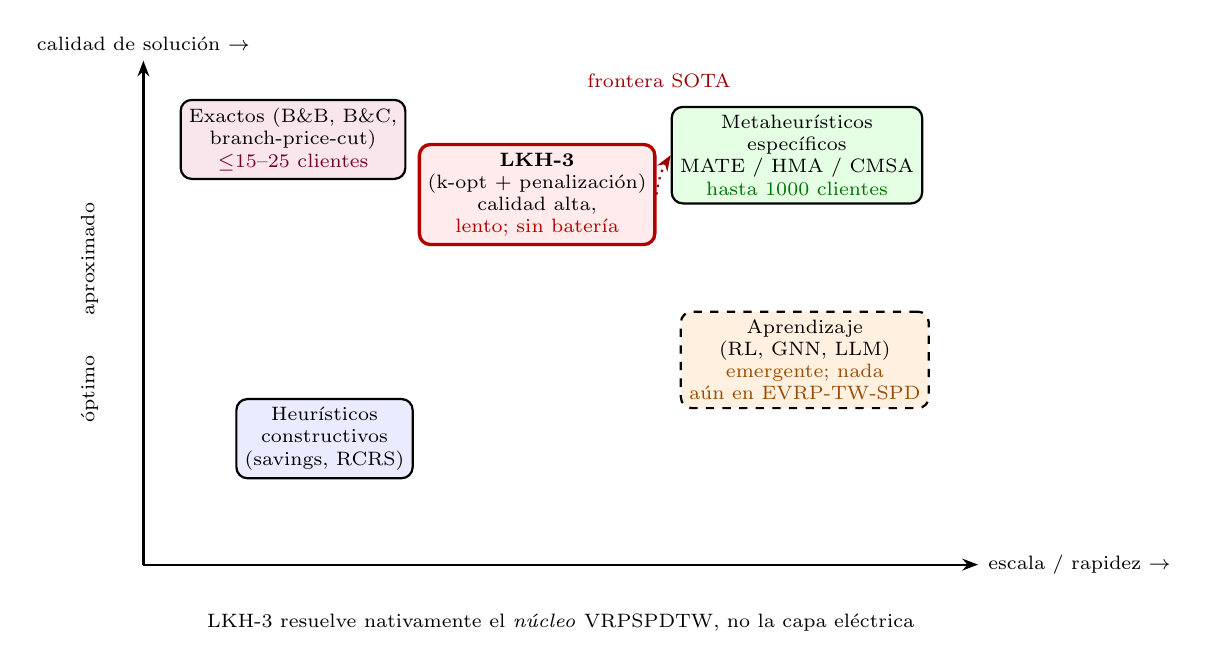
\begin{tikzpicture}[
  >={Stealth[length=2mm]},
  fam/.style={rounded corners,draw,thick,align=center,font=\scriptsize,inner sep=3pt},
  lkh/.style={rounded corners,draw=red!70!black,very thick,fill=red!8,align=center,
              font=\scriptsize,inner sep=3pt}
]
  % ejes
  \draw[->,thick] (0,0) -- (10.6,0) node[right,font=\scriptsize,align=center] {escala / rapidez $\rightarrow$};
  \draw[->,thick] (0,0) -- (0,6.4) node[above,font=\scriptsize] {calidad de soluci\'on $\rightarrow$};
  \node[font=\scriptsize,rotate=90,anchor=south] at (-0.45,3.2) {\'optimo \;\;\;\; aproximado};

  % familias de metodos (x = escala/rapidez, y = calidad)
  \node[fam,fill=purple!10] (exact) at (1.9,5.4)
       {Exactos (B\&B, B\&C,\\ branch-price-cut)\\ \textcolor{purple!60!black}{$\le$15--25 clientes}};
  \node[fam,fill=blue!8]   (constr) at (2.3,1.6)
       {Heur\'isticos\\ constructivos\\ (savings, RCRS)};
  \node[lkh] (lkh) at (5.0,4.7)
       {\textbf{LKH-3}\\ (k-opt + penalizaci\'on)\\ calidad alta,\\
        \textcolor{red!70!black}{lento; sin bater\'ia}};
  \node[fam,fill=green!10] (meta) at (8.3,5.2)
       {Metaheur\'isticos\\ espec\'ificos\\ MATE / HMA / CMSA\\ \textcolor{green!45!black}{hasta 1000 clientes}};
  \node[fam,fill=orange!12,dashed] (ml) at (8.4,2.6)
       {Aprendizaje\\ (RL, GNN, LLM)\\ \textcolor{orange!60!black}{emergente; nada}\\
        \textcolor{orange!60!black}{a\'un en EVRP-TW-SPD}};

  % flecha de la tendencia
  \draw[->,thick,red!60!black,dotted] (lkh.east) to[bend left=12] (meta.west);
  \node[font=\scriptsize,red!60!black] at (6.55,6.15) {frontera SOTA};

  % nota: LKH-3 resuelve solo el nucleo VRPSPDTW
  \node[font=\scriptsize,align=center,anchor=north] at (5.3,-0.5)
       {LKH-3 resuelve nativamente el \emph{n\'ucleo} VRPSPDTW, no la capa el\'ectrica};
\end{tikzpicture}

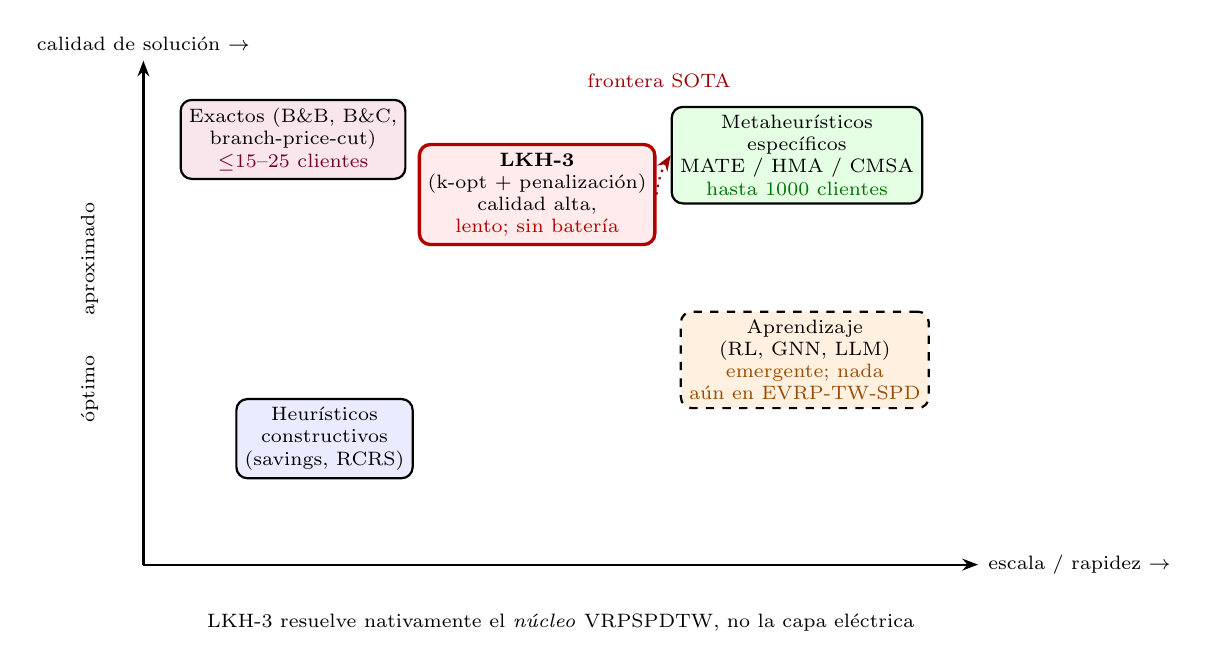
\begin{tikzpicture}[
  >={Stealth[length=2mm]},
  fam/.style={rounded corners,draw,thick,align=center,font=\scriptsize,inner sep=3pt},
  lkh/.style={rounded corners,draw=red!70!black,very thick,fill=red!8,align=center,
              font=\scriptsize,inner sep=3pt}
]
  % ejes
  \draw[->,thick] (0,0) -- (10.6,0) node[right,font=\scriptsize,align=center] {escala / rapidez $\rightarrow$};
  \draw[->,thick] (0,0) -- (0,6.4) node[above,font=\scriptsize] {calidad de soluci\'on $\rightarrow$};
  \node[font=\scriptsize,rotate=90,anchor=south] at (-0.45,3.2) {\'optimo \;\;\;\; aproximado};

  % familias de metodos (x = escala/rapidez, y = calidad)
  \node[fam,fill=purple!10] (exact) at (1.9,5.4)
       {Exactos (B\&B, B\&C,\\ branch-price-cut)\\ \textcolor{purple!60!black}{$\le$15--25 clientes}};
  \node[fam,fill=blue!8]   (constr) at (2.3,1.6)
       {Heur\'isticos\\ constructivos\\ (savings, RCRS)};
  \node[lkh] (lkh) at (5.0,4.7)
       {\textbf{LKH-3}\\ (k-opt + penalizaci\'on)\\ calidad alta,\\
        \textcolor{red!70!black}{lento; sin bater\'ia}};
  \node[fam,fill=green!10] (meta) at (8.3,5.2)
       {Metaheur\'isticos\\ espec\'ificos\\ MATE / HMA / CMSA\\ \textcolor{green!45!black}{hasta 1000 clientes}};
  \node[fam,fill=orange!12,dashed] (ml) at (8.4,2.6)
       {Aprendizaje\\ (RL, GNN, LLM)\\ \textcolor{orange!60!black}{emergente; nada}\\
        \textcolor{orange!60!black}{a\'un en EVRP-TW-SPD}};

  % flecha de la tendencia
  \draw[->,thick,red!60!black,dotted] (lkh.east) to[bend left=12] (meta.west);
  \node[font=\scriptsize,red!60!black] at (6.55,6.15) {frontera SOTA};

  % nota: LKH-3 resuelve solo el nucleo VRPSPDTW
  \node[font=\scriptsize,align=center,anchor=north] at (5.3,-0.5)
       {LKH-3 resuelve nativamente el \emph{n\'ucleo} VRPSPDTW, no la capa el\'ectrica};
\end{tikzpicture}

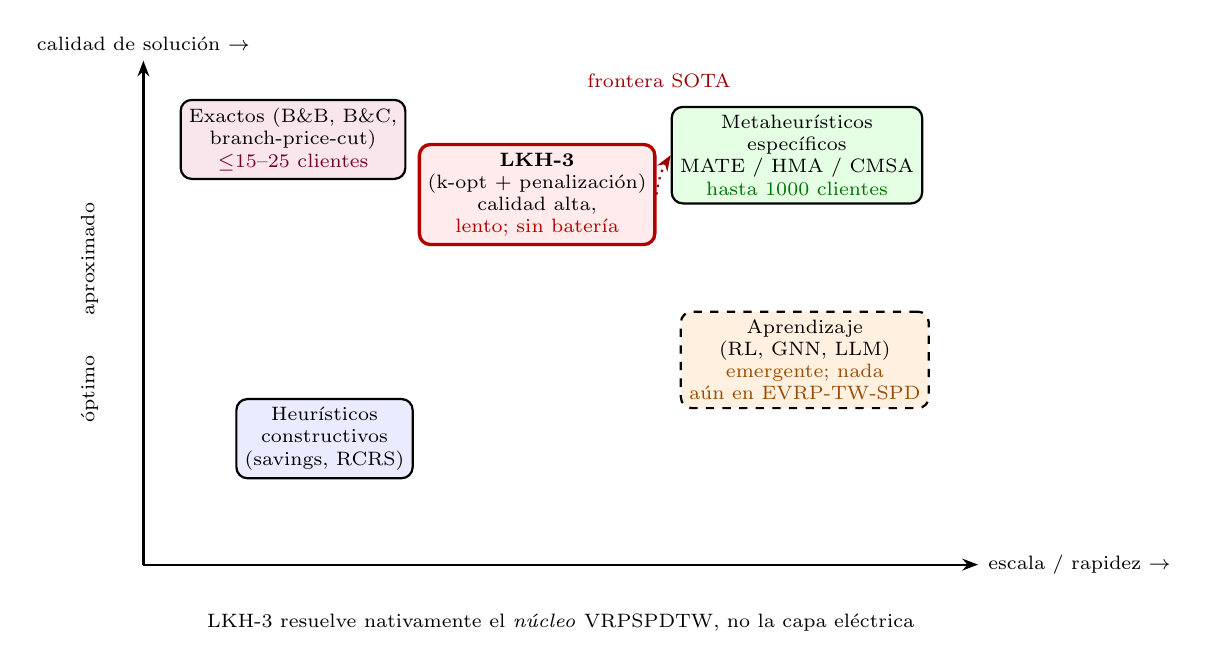
\begin{tikzpicture}[
  >={Stealth[length=2mm]},
  fam/.style={rounded corners,draw,thick,align=center,font=\scriptsize,inner sep=3pt},
  lkh/.style={rounded corners,draw=red!70!black,very thick,fill=red!8,align=center,
              font=\scriptsize,inner sep=3pt}
]
  % ejes
  \draw[->,thick] (0,0) -- (10.6,0) node[right,font=\scriptsize,align=center] {escala / rapidez $\rightarrow$};
  \draw[->,thick] (0,0) -- (0,6.4) node[above,font=\scriptsize] {calidad de soluci\'on $\rightarrow$};
  \node[font=\scriptsize,rotate=90,anchor=south] at (-0.45,3.2) {\'optimo \;\;\;\; aproximado};

  % familias de metodos (x = escala/rapidez, y = calidad)
  \node[fam,fill=purple!10] (exact) at (1.9,5.4)
       {Exactos (B\&B, B\&C,\\ branch-price-cut)\\ \textcolor{purple!60!black}{$\le$15--25 clientes}};
  \node[fam,fill=blue!8]   (constr) at (2.3,1.6)
       {Heur\'isticos\\ constructivos\\ (savings, RCRS)};
  \node[lkh] (lkh) at (5.0,4.7)
       {\textbf{LKH-3}\\ (k-opt + penalizaci\'on)\\ calidad alta,\\
        \textcolor{red!70!black}{lento; sin bater\'ia}};
  \node[fam,fill=green!10] (meta) at (8.3,5.2)
       {Metaheur\'isticos\\ espec\'ificos\\ MATE / HMA / CMSA\\ \textcolor{green!45!black}{hasta 1000 clientes}};
  \node[fam,fill=orange!12,dashed] (ml) at (8.4,2.6)
       {Aprendizaje\\ (RL, GNN, LLM)\\ \textcolor{orange!60!black}{emergente; nada}\\
        \textcolor{orange!60!black}{a\'un en EVRP-TW-SPD}};

  % flecha de la tendencia
  \draw[->,thick,red!60!black,dotted] (lkh.east) to[bend left=12] (meta.west);
  \node[font=\scriptsize,red!60!black] at (6.55,6.15) {frontera SOTA};

  % nota: LKH-3 resuelve solo el nucleo VRPSPDTW
  \node[font=\scriptsize,align=center,anchor=north] at (5.3,-0.5)
       {LKH-3 resuelve nativamente el \emph{n\'ucleo} VRPSPDTW, no la capa el\'ectrica};
\end{tikzpicture}
}
  \caption{Mapa del estado del arte. LKH-3 alcanza alta calidad en el n\'ucleo
  VRPSPDTW pero es lento y no cubre la capa el\'ectrica; la frontera en
  VRPSPDTW-E la marcan metaheur\'isticos espec\'ificos (memet\'icos, CMSA), con
  el aprendizaje a\'un emergente.}
  \label{fig:mapa}
\end{figure*}

\subsection{Capa A: VRPSPD / VRPSPDTW (el n\'ucleo)}
Los m\'etodos \emph{exactos} (branch-and-cut, branch-and-price) resuelven solo
instancias peque\~nas. Entre los \emph{constructivos} destaca la heur\'istica
RCRS (\emph{residual capacity and radial surcharge}) \cite{dethloff2001}, base de
inicializaci\'on de muchos metaheur\'isticos. Para VRPSPD se han aplicado
b\'usqueda tab\'u reactiva \cite{wassan2008}, recocido simulado, GA, ACO y PSO.
Para VRPSPDTW, la l\'inea m\'as activa parte del GA coevolutivo de Wang y Chen
\cite{wangchen2012} (que estableci\'o el benchmark de referencia) y avanza por
recocido simulado paralelo, VNS con tab\'u y \emph{adaptive large neighborhood
search} con \emph{path-relinking}, hasta el algoritmo \emph{memet\'ico} MATE
\cite{liu2021mate}, actual estado del arte del problema base: combina
inicializaci\'on por diversidad, un \emph{crossover} de ensamblaje de rutas con
inserci\'on por arrepentimiento, b\'usqueda local multi-operador (2-opt, 2-opt*,
or-opt, swap) y evaluaci\'on de movimientos en $O(1)$.

\subsection{Capa B: EVRP / EVRPTW (la dimensi\'on el\'ectrica)}
Erdo\u{g}an y Miller-Hooks \cite{erdogan2012green} introdujeron el \emph{Green
VRP} con estaciones de recarga, y Schneider \emph{et al.}
\cite{schneider2014evrptw} el EVRPTW, con un h\'ibrido VNS+tab\'u y los
benchmarks de referencia. Desaulniers \emph{et al.} \cite{desaulniers2016exact}
aportaron algoritmos exactos \emph{branch-price-and-cut}. La \emph{recarga
parcial} ---clave para ventanas estrechas--- fue desarrollada por Felipe
\emph{et al.} \cite{felipe2014} y Keskin y \c{C}atay \cite{keskin2016partial},
con extensiones a cargadores r\'apidos \cite{keskin2018fast} y esperas
estoc\'asticas \cite{keskin2021stochastic}. Existen revisiones amplias del \'area
\cite{kucukoglu2021review,qin2021review}.

\subsection{Capa C: la fusi\'on VRPSPDTW-E}
La literatura es escasa y reciente (toda posterior a 2020). Akbay \emph{et al.}
\cite{akbay2022cmsa} \emph{introdujeron} el problema, dieron su MILP y propusieron
una matheur\'istica \emph{Construct--Merge--Solve--Adapt} (Adapt-CMSA),
mejorada luego con modelos de \emph{set covering} \cite{akbay2024setcov}. Feng
\emph{et al.} \cite{feng2023admm} aplicaron ADMM en instancias peque\~nas con
recarga completa. El estado del arte actual es el algoritmo memet\'ico h\'ibrido
(HMA) de Zheng \emph{et al.} \cite{zheng2025hma}, que combina \emph{large
neighborhood search}, b\'usqueda memet\'ica e inserci\'on de estaciones
paralelo-secuencial, escalando a $1000$ clientes.

\subsection{Capa D: aprendizaje}
El aprendizaje por refuerzo y las redes neuronales se aplican a VRPs m\'as
simples \cite{wang2025drlalns,liu2023neural}; la tendencia con LKH es
\emph{guiarlo o acelerarlo} (p.\,ej.\ variantes reforzadas) m\'as que
reemplazarlo. Para el VRPSPDTW-E, sin embargo, no existen a\'un m\'etodos de
aprendizaje maduros: es una brecha clara.

%=======================================================================
\section{LKH-3 aplicado al problema}\label{sec:lkh}
%=======================================================================
\subsection{Mec\'anica}
LKH-3 \cite{helsgaun2017lkh3} extiende el algoritmo de Lin--Kernighan
\cite{linkernighan1973,helsgaun2000lkh,helsgaun2009kopt} a TSP/VRP restringidos
mediante dos ideas. Primero, \emph{transforma} todo problema a un TSP sim\'etrico:
los problemas con ventanas se tratan como asim\'etricos y luego se simetrizan, y
una flota de $m$ veh\'iculos se modela a\~nadiendo $m-1$ copias del dep\'osito.
Segundo, maneja las restricciones con \emph{funciones de penalizaci\'on}: a cada
tour se le asocia un par $(P,C)$ ---penalizaci\'on por violaci\'on y costo--- y
se ordena lexicogr\'aficamente ($P$ primero, $C$ despu\'es), lo que permite
buscar en el espacio infactible y converger a factibilidad. Para VRPSPD, el
formato de entrada especifica directamente los tama\~nos de recogida y entrega de
cada nodo, y la penalizaci\'on acumula la violaci\'on de capacidad (carga no
mon\'otona que excede $C$) y de ventanas. Como la evaluaci\'on de la
penalizaci\'on es $O(N)$, LKH-3 usa un generador de 5-opt especializado para
limitar el n\'umero de movimientos.

\subsection{Resultados reportados}
Helsgaun reporta que, sobre instancias de la literatura, LKH-3 \emph{mejora o
iguala} la mejor soluci\'on conocida (BKS) en VRPSPDTW con notable frecuencia
(Tabla~\ref{tab:lkh}). Sin embargo, su calidad es m\'as irregular en VRPSPD (sin
ventanas).

\begin{table}[t]
  \centering
  \caption{Resultados de LKH-3 vs.\ la mejor soluci\'on conocida (BKS),
  reportados por Helsgaun \cite{helsgaun2017lkh3}.}
  \label{tab:lkh}
  \renewcommand{\arraystretch}{1.15}
  \begin{tabular}{@{}lcccc@{}}
    \toprule
    Problema & Instancias & $<$ BKS & $=$ BKS & $>$ BKS \\
    \midrule
    \textbf{VRPSPDTW} & 68  & \textbf{46} & 20  & 2  \\
    VRPSPD            & 266 & 20          & 148 & 98 \\
    CVRPTW (ref.)     & 405 & 2           & 302 & 101 \\
    \bottomrule
  \end{tabular}
\end{table}

\subsection{Posicionamiento cr\'itico}
\textbf{Fortalezas:} motor de b\'usqueda local general y potente; el esquema
$(P,C)$ es modular (a\~nadir una restricci\'on es a\~nadir un t\'ermino de
penalizaci\'on); calidad competitiva e incluso nuevas BKS en VRPSPDTW.
\textbf{Limitaciones:} (i)~\emph{tiempo}: la penalizaci\'on $O(N)$ lo vuelve
lento; Liu \emph{et al.} \cite{liu2021mate} reportan que LKH~3.0 tardaba
``t\'ipicamente dos d\'ias'' en hallar una soluci\'on \emph{factible} de
VRPSPDTW, por lo que lo descartaron de su comparaci\'on; (ii)~\emph{sin capa
el\'ectrica}: el solver no modela SoC, estaciones ni recarga;
(iii)~las estaciones son nodos \emph{opcionales y repetibles}, en tensi\'on con
el paradigma TSP de visitar cada nodo una vez; y (iv)~la recarga $q$ es una
variable \emph{continua}, ajena a los movimientos combinatorios $k$-opt.

\subsection{C\'omo extender LKH-3 al VRPSPDTW-E}
Apoy\'andonos en que \emph{retirar las estaciones de una soluci\'on el\'ectrica
factible deja una soluci\'on factible del VRPSPDTW} \cite{zheng2025hma},
proponemos como l\'inea conceptual (Fig.~\ref{fig:via1}) usar LKH-3 como
\emph{motor base} del n\'ucleo VRPSPDTW y envolverlo con una capa externa que
inserte estaciones y reparta la recarga parcial ---el mismo patr\'on que emplean
HMA \cite{zheng2025hma} y CMSA \cite{akbay2022cmsa}. Es la v\'ia m\'as coherente
con la filosof\'ia de LKH-3, pues no requiere alterar su n\'ucleo y aprovecha su
fortaleza en el subproblema combinatorio. Alternativas m\'as invasivas ---a\~nadir
una penalizaci\'on de bater\'ia y pre-replicar estaciones como nodos opcionales,
o duplicar nodos por niveles de SoC--- son posibles pero menos naturales por la
variable continua de recarga.

\begin{figure}[t]
  \centering
  \resizebox{\columnwidth}{!}{% fig3_via1.tex  — Figura 3: "Via 1" — LKH-3 como motor base + capa de recarga
% Requiere: \usetikzlibrary{positioning,arrows.meta,shapes.geometric}
% Se incluye con:  % fig3_via1.tex  — Figura 3: "Via 1" — LKH-3 como motor base + capa de recarga
% Requiere: \usetikzlibrary{positioning,arrows.meta,shapes.geometric}
% Se incluye con:  % fig3_via1.tex  — Figura 3: "Via 1" — LKH-3 como motor base + capa de recarga
% Requiere: \usetikzlibrary{positioning,arrows.meta,shapes.geometric}
% Se incluye con:  \input{fig3_via1}
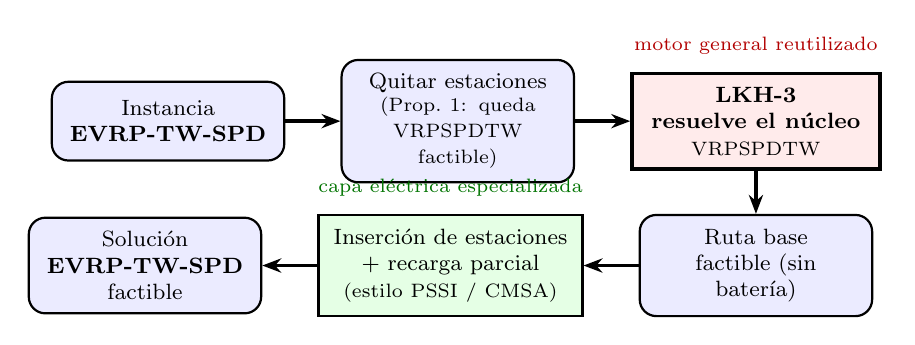
\begin{tikzpicture}[
  >={Stealth[length=2.4mm]},
  node distance=5.5mm and 7mm,
  io/.style={rounded corners=6pt,draw,thick,fill=blue!8,align=center,
             font=\footnotesize,inner sep=5pt,minimum height=10mm,text width=26mm},
  eng/.style={draw,very thick,fill=red!8,align=center,font=\footnotesize\bfseries,
              inner sep=5pt,minimum height=12mm,text width=28mm},
  rep/.style={draw,thick,fill=green!10,align=center,font=\footnotesize,
              inner sep=5pt,minimum height=12mm,text width=30mm},
  flow/.style={->,very thick}
]
  \node[io]  (in)   {Instancia\\ \textbf{EVRP-TW-SPD}};
  \node[io,right=of in] (strip) {Quitar estaciones\\ \scriptsize(Prop.~1: queda\\ VRPSPDTW factible)};
  \node[eng,right=of strip] (lkh) {LKH-3\\ resuelve el n\'ucleo\\ \textmd{\scriptsize VRPSPDTW}};
  \node[io,below=of lkh] (route) {Ruta base\\ factible (sin\\ bater\'ia)};
  \node[rep,left=of route] (insert) {Inserci\'on de estaciones\\ + recarga parcial\\ \scriptsize(estilo PSSI / CMSA)};
  \node[io,left=of insert] (out) {Soluci\'on\\ \textbf{EVRP-TW-SPD}\\ factible};

  \draw[flow] (in) -- (strip);
  \draw[flow] (strip) -- (lkh);
  \draw[flow] (lkh) -- (route);
  \draw[flow] (route) -- (insert);
  \draw[flow] (insert) -- (out);

  \node[font=\scriptsize,align=center,red!70!black] at (lkh.north) [above=1mm]
       {motor general reutilizado};
  \node[font=\scriptsize,align=center,green!45!black] at (insert.north) [above=1mm]
       {capa el\'ectrica especializada};
\end{tikzpicture}

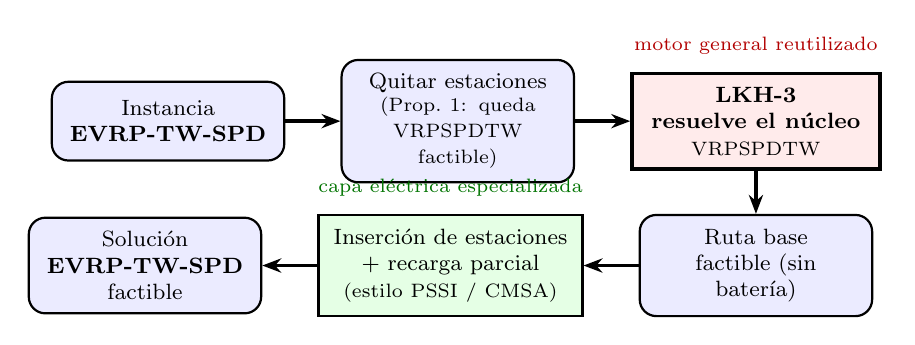
\begin{tikzpicture}[
  >={Stealth[length=2.4mm]},
  node distance=5.5mm and 7mm,
  io/.style={rounded corners=6pt,draw,thick,fill=blue!8,align=center,
             font=\footnotesize,inner sep=5pt,minimum height=10mm,text width=26mm},
  eng/.style={draw,very thick,fill=red!8,align=center,font=\footnotesize\bfseries,
              inner sep=5pt,minimum height=12mm,text width=28mm},
  rep/.style={draw,thick,fill=green!10,align=center,font=\footnotesize,
              inner sep=5pt,minimum height=12mm,text width=30mm},
  flow/.style={->,very thick}
]
  \node[io]  (in)   {Instancia\\ \textbf{EVRP-TW-SPD}};
  \node[io,right=of in] (strip) {Quitar estaciones\\ \scriptsize(Prop.~1: queda\\ VRPSPDTW factible)};
  \node[eng,right=of strip] (lkh) {LKH-3\\ resuelve el n\'ucleo\\ \textmd{\scriptsize VRPSPDTW}};
  \node[io,below=of lkh] (route) {Ruta base\\ factible (sin\\ bater\'ia)};
  \node[rep,left=of route] (insert) {Inserci\'on de estaciones\\ + recarga parcial\\ \scriptsize(estilo PSSI / CMSA)};
  \node[io,left=of insert] (out) {Soluci\'on\\ \textbf{EVRP-TW-SPD}\\ factible};

  \draw[flow] (in) -- (strip);
  \draw[flow] (strip) -- (lkh);
  \draw[flow] (lkh) -- (route);
  \draw[flow] (route) -- (insert);
  \draw[flow] (insert) -- (out);

  \node[font=\scriptsize,align=center,red!70!black] at (lkh.north) [above=1mm]
       {motor general reutilizado};
  \node[font=\scriptsize,align=center,green!45!black] at (insert.north) [above=1mm]
       {capa el\'ectrica especializada};
\end{tikzpicture}

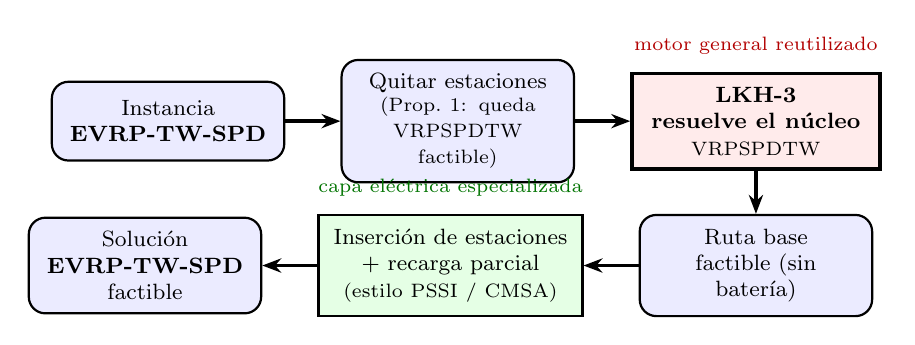
\begin{tikzpicture}[
  >={Stealth[length=2.4mm]},
  node distance=5.5mm and 7mm,
  io/.style={rounded corners=6pt,draw,thick,fill=blue!8,align=center,
             font=\footnotesize,inner sep=5pt,minimum height=10mm,text width=26mm},
  eng/.style={draw,very thick,fill=red!8,align=center,font=\footnotesize\bfseries,
              inner sep=5pt,minimum height=12mm,text width=28mm},
  rep/.style={draw,thick,fill=green!10,align=center,font=\footnotesize,
              inner sep=5pt,minimum height=12mm,text width=30mm},
  flow/.style={->,very thick}
]
  \node[io]  (in)   {Instancia\\ \textbf{EVRP-TW-SPD}};
  \node[io,right=of in] (strip) {Quitar estaciones\\ \scriptsize(Prop.~1: queda\\ VRPSPDTW factible)};
  \node[eng,right=of strip] (lkh) {LKH-3\\ resuelve el n\'ucleo\\ \textmd{\scriptsize VRPSPDTW}};
  \node[io,below=of lkh] (route) {Ruta base\\ factible (sin\\ bater\'ia)};
  \node[rep,left=of route] (insert) {Inserci\'on de estaciones\\ + recarga parcial\\ \scriptsize(estilo PSSI / CMSA)};
  \node[io,left=of insert] (out) {Soluci\'on\\ \textbf{EVRP-TW-SPD}\\ factible};

  \draw[flow] (in) -- (strip);
  \draw[flow] (strip) -- (lkh);
  \draw[flow] (lkh) -- (route);
  \draw[flow] (route) -- (insert);
  \draw[flow] (insert) -- (out);

  \node[font=\scriptsize,align=center,red!70!black] at (lkh.north) [above=1mm]
       {motor general reutilizado};
  \node[font=\scriptsize,align=center,green!45!black] at (insert.north) [above=1mm]
       {capa el\'ectrica especializada};
\end{tikzpicture}
}
  \caption{Esquema conceptual: LKH-3 como motor del n\'ucleo VRPSPDTW, envuelto
  en una capa especializada de inserci\'on de estaciones y recarga parcial.}
  \label{fig:via1}
\end{figure}

%=======================================================================
\section{Discusi\'on y trabajo futuro}\label{sec:gaps}
%=======================================================================
El VRPSPDTW-E es un nicho abierto y reciente. Persisten varias brechas.
\emph{De m\'etodo:} los exactos no escalan m\'as all\'a de $\sim15$ clientes y
no hay m\'etodos de aprendizaje maduros para esta variante. \emph{De benchmark:}
los conjuntos est\'andar llegan a $100$ clientes, lejos de las escalas reales.
\emph{De modelado:} la recarga real es no lineal, hay colas estoc\'asticas en
estaciones, degradaci\'on de bater\'ia y precios por franja horaria. En esta
l\'inea, nuestra formulaci\'on \emph{incorpora} un \emph{consumo energ\'etico
dependiente de la carga} ($h_0+h_1\!\cdot\!\text{carga}$), tanto en el objetivo
como en la din\'amica de bater\'ia, a diferencia del consumo constante habitual
en la literatura; esto captura la interacci\'on entre el SPD ---donde la carga
var\'ia de forma no mon\'otona--- y el gasto energ\'etico. Refinarlo con curvas de
carga no lineales y consumo dependiente de velocidad o pendiente queda como
trabajo futuro. Finalmente, no existe una integraci\'on de LKH-3
con la capa el\'ectrica: la Fig.~\ref{fig:via1} la esboza como l\'inea futura. La
tendencia general apunta a \emph{h\'ibridos} que combinen un motor de b\'usqueda
local fuerte (como LKH-3) con reparaci\'on el\'ectrica especializada y, cada vez
m\'as, con componentes de aprendizaje para guiar la b\'usqueda a escala
industrial.

%=======================================================================
\section*{Declaraci\'on de uso de IA}
%=======================================================================
Se utiliz\'o un asistente de IA generativa (Kimi K2.7) como apoyo en la
\emph{b\'usqueda y organizaci\'on bibliogr\'afica}, la \emph{extracci\'on de
informaci\'on} de las fuentes primarias, la \emph{generaci\'on de esquemas
iniciales} y figuras, y la \emph{edici\'on de redacci\'on}. La estructura
anal\'itica, el posicionamiento cr\'itico de LKH-3 y la discusi\'on son obra del
grupo. Todas las referencias citadas fueron verificadas y le\'idas por al menos
un integrante.

%=======================================================================
\bibliographystyle{IEEEtran}
\bibliography{referencias}
%=======================================================================

\end{document}
